i%%%%%%%%%%%%%%%%%%%%%%%%%%%%%%%%%%%%%%%%%%%%%%%%%%%%%%%%%%%%%%%%
%                                                               %
%                       Legal Notice                            %
%                                                               %
% This document is copyright (C) Jason Gobat & Darren Atkinson	%
%                                                               %
%%%%%%%%%%%%%%%%%%%%%%%%%%%%%%%%%%%%%%%%%%%%%%%%%%%%%%%%%%%%%%%%%

\newpage{\pagestyle{empty}\cleardoublepage}

\chapter{The {\em velvet} Application}
\label{velvet}

\section{Introduction to the {\em velvet} GUI}
\label{velvet.intro}

{\em velvet} was designed as the primary user interface to the \felt{}
system.  Generally, if the \felt{} system can solve a given problem,
you will find it easier to specify, solve and analyze the results for that 
problem right within the {\em velvet} GUI.  {\em velvet} embodies all of
the mathematical features of \felt{}, as well as graphical pre- and 
post-processing and element generation.

The main {\em velvet} window consists of three major areas 
(Figure~\ref{velvet.main}).  The first is the 
list of menu buttons down the left side of the window.  This is the main 
control area for all of the operations in {\em velvet}.  The second is the 
command/status line across the bottom of the window.  This line is used to 
display messages and for keyboard based input.
The third is the drawing area, which occupies most 
of the window.  This is the area in which you can dynamically define and 
interact with the \felt{} problem. 

\begin{figure}
\begin{center}
 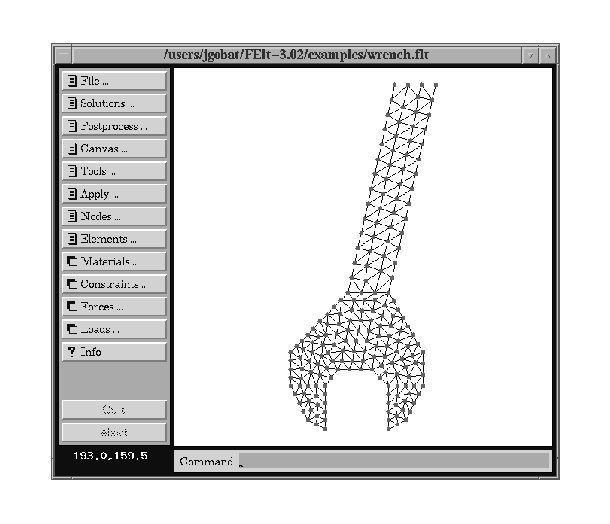
\includegraphics[width=6.0in]{figures/velvet_main}
\end{center}
\caption{Main {\em velvet} drawing area with an interesting sample problem.}
\label{velvet.main}
\end{figure}

The menus are used to define everything about a problem (nodes, elements, 
forces, constraints, material properties, distributed loads), to configure 
{\em velvet}, to use the drawing tools, to configure the drawing area and to 
save, open and solve problems.  

\section{General features of the interface}

Many of the interface modules that you will see in {\em velvet} look
very similar to one another.  Becoming familiar with a few basic operations
that are common across all of these modules will allow you to use
{\em velvet} much more easily and flexibly.

In general, clicking an {\bf accept} button will register the current state
of a dialog with the rest of the application.  Say you have a dialog
with a few toggle buttons and a couple of entry blanks. You could
change the button states and type things into the entry blanks all you
wanted without actually affecting the rest of {\em velvet}.  Once you
click {\bf accept}, however, all of your changes become effective.  This
behavior is similar to an {\bf okay} button in many GUIs; the difference
is that {\bf accept} will not cause the dialog box to disappear.  You will
need to click the {\bf dismiss} button to do that.  

Where there is a {\bf help} button, you can click and hold it to view
a brief help message about that dialog.  In some dialogs, additional help is 
available by clicking and holding over special labels.  This type of
help will be discussed in more detail later.

A final factor that is common across GUI components is the idea of multiple
mechanisms.  In general, there are three different ways that you can
perform an action in {\em velvet}.  The first is by the standard
point, click, and drag operations of the mouse.  The second is through 
keyboard shortcuts.  The third is by entering commands or data into
the command window at the bottom of the main drawing area.  For the most
part, we will limit our initial discussion to the mouse operations.
Section~\ref{velvet.keyboard} presents a summary of the equivalencies
between the different interface methods for those of you who want to 
become {\em velvet} power users.  For now, it should be enough to know
that whenever {\em velvet} prompts you for a coordinate you can
either click in the drawing area or type in an {\tt x,y} pair in the
command window (followed by a \key{return} of course). 
Similarly if you are being asked to select an element
or node; you can either type in the appropriate number or click on 
the appropriate object.

\section{Working with files}

If you already have a \felt{} input file defined, the easiest way to
start working with that file is by specifying the filename on the 
shell command line when you invoke {\em velvet}.  For example, 
\begin{screen}
 \begin{verbatim}
% velvet foo.flt
 \end{verbatim}
\end{screen}
Will start {\em velvet} and automatically load in the file {\tt foo.flt}.
The drawing area will be initially configured to some reasonable
values to allow you to view the entire problem.  If this file was
saved from {\em velvet} then it will contain special sections that describe
all of the figures and the configuration of the drawing area when the file
was saved.  {\em velvet} will use this information to reconstruct all of
these things exactly as you left them.

Alternatively, you can invoke {\em velvet} with no filename and then use 
the standard {\em velvet} file selection mechanism to load a file.
Select {\bf open} from the {\bf file} menu.  This will bring up a dialog
box that looks something like the one shown in Figure~\ref{velvet.file}.  
This dialog
is the standard way for you to specify filenames (either for loading or 
saving problem files or graphical dumps).  Within this dialog you
can choose a file either by typing into the entry box at the top of
the dialog or by clicking on a filename in the list with the first mouse
button.  Clicking {\bf okay} will finalize your selection.  You can 
maneuver through directories by selecting them and clicking {\bf okay}
just like files.  
An alternative to selecting an entry then clicking the {\bf okay} button 
is to click on list entries with the middle mouse button.  This will instantly 
select that entry (or move to that directory).  Clicking the {\bf cancel}
button will dismiss the file selection dialog without making a selection.

\begin{figure}
\begin{center}
 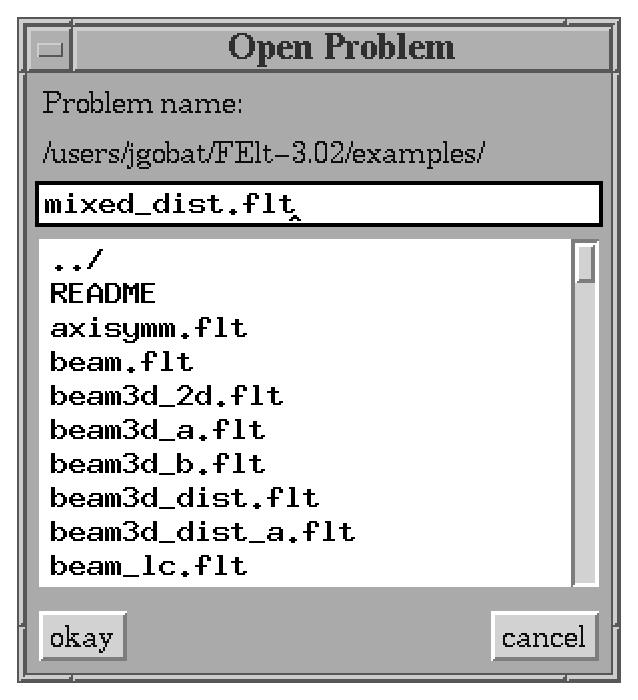
\includegraphics[width=2.25in]{figures/velvet_file}
\end{center}
\caption{The {\em velvet} file selection mechanism.}
\label{velvet.file}
\end{figure}

Additional entries on the {\bf file} menu should appear familiar to
most users of modern GUI applications.  Choosing {\bf new} will erase
the current problem and allow you to start with a blank slate.  You'll
be prompted if there is a chance that you might lose some unsaved changes
to the current problem.  {\bf save} does just what it says; if the current
problem does not have a filename already associated with it, choosing
{\bf save} acts like {\bf save as}, otherwise it will silently save
the current state of the problem to the associated file.  The current filename
is always displayed as the title in the window manager title bar. 
{\bf save as} allows you to name the file that the problem will be saved to.
After saving through a {\bf save as} action, this filename becomes the
current filename for this problem.  The {\bf restore} option is equivalent
to selecting {\bf open} and choosing the current input file (i.e., it simply
reloads the currently named input file).  {\bf exit} quits {\em velvet}
entirely; you will be prompted if you have unsaved changes.

Note that when {\em velvet} saves a file, it will consist of the standard
sections of a \felt{} file plus special sections that describe the appearance
of the drawing area.  These ancillary sections contain information
that allows {\em velvet} to reconstruct the drawing area (including tool
figures, canvas configuration options and zoom state) when the corresponding
\felt{} file is loaded 
back into {\em velvet}.  You should never have to worry about whether or not
such information exists.  If a file with these sections is run through
{\em felt} the information simply will be ignored.  If the information 
does not exist
and you load the file into {\em velvet} then {\em velvet} simply will make
a best guess as to how to configure the main canvas area.  The advantage to
having such a plain text description of the drawing area is that you can change
this information outside of {\em velvet} if you want to make quick changes to 
the problem appearance but do not want to load {\em velvet} explicitly.  Such
an arrangement also allows you to easily create defaults files which you
can use to start-up {\em velvet} with your preferred configuration.

\section{Configuring the drawing area}
\subsection{Basic controls}

The primary means for setting up the drawing area is through the 
{\bf configure} dialog under the {\bf canvas} menu 
(Figure~\ref{velvet.configure}).  The left side of this dialog deals primarily 
with the minimum and maximum coordinates of the drawing area, the snap size 
and the grid size.  The right side allows you to specify the colors and fonts 
to use for the different objects that appear in the drawing area.
The label font is used for node and element numbers. 
Also included on the {\bf configure} dialog are toggle buttons to control
the status of snap, grid, element numbering and node numbering.
Note that these four toggles are also available by selecting the appropriate 
entry right on the {\bf canvas} menu.  You must click {\bf accept} to
make any of your changes active.   

\begin{figure}
\begin{center}
 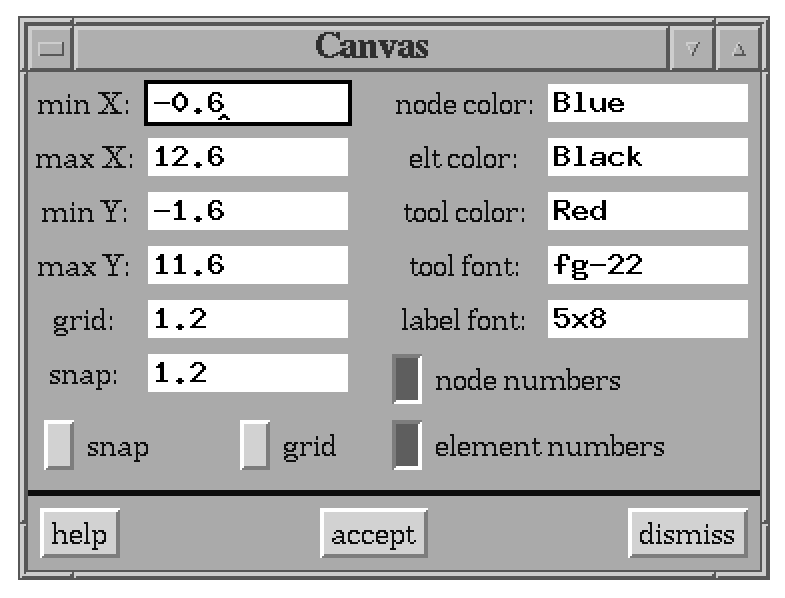
\includegraphics[width=2.91in]{figures/velvet_configure}
\end{center}
\caption{The configuration dialog box.}
\label{velvet.configure}
\end{figure}

As mentioned above, the {\bf snap} and {\bf grid} options act as toggle 
switches for these common drawing aids.  For those unfamiliar with these
terms, {\bf grid} produces a ruled grid across the drawing area to help you 
locate yourself as you work and {\bf snap} insures that mouse selected 
coordinates will fall on regular fractions (i.e., a snap size of 0.25
insures that all of your selections will be rounded to the nearest
quarter unit).  Note that the
grid size (the spacing of the rulings on the screen) and the snap size (the
fraction to which your selected coordinates will be automatically rounded) are
controlled separately by entries in the {\bf configure} dialog.  
The {\bf node numbers} option acts as a 
toggle switch for node numbering - in a crowded problem, visible node numbers 
may not be helpful as they can tend to clutter the display.  The same
is true for the {\bf element numbers} option.  
A check mark will appear next to the menu entry if the option is enabled.  

\subsection{Object coloring}
Beyond the basic node color and element color controls provided in the 
canvas configuration dialog (Figure~\ref{velvet.configure}), {\em velvet}
also allows you to assign unique colors to individual forces, constraints,
material properties and distributed loads.  Selecting {\bf color control}
from the {\bf canvas} menu will pop-up the colors dialog shown in 
Figure~\ref{velvet.colors}.  The four smaller scrolled lists on the left
list all of the attributable objects (materials, distributed loads, 
constraints, forces; see section~\ref{velvet.drawing_defining}) defined
in the current problem.  The larger list running down the right side lists
the available colors.  By highlighting an entry in one of the four object
lists you can assign a color to that object.  

\begin{figure}
\begin{center}
 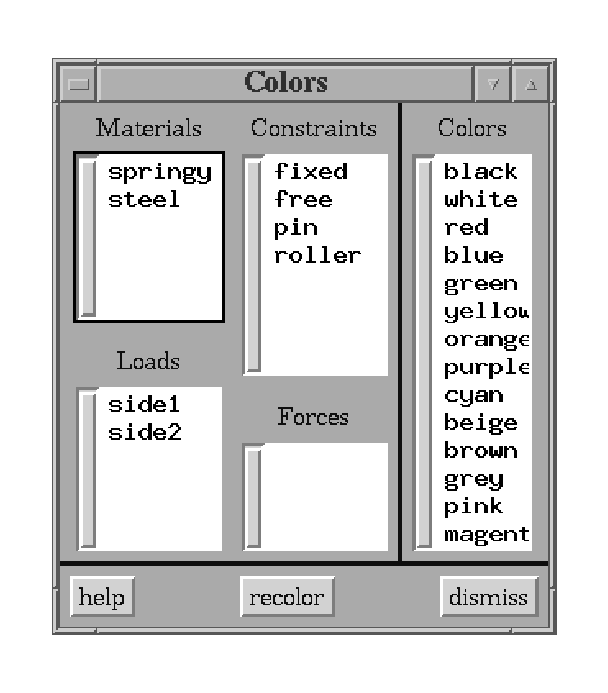
\includegraphics[width=2.49in]{figures/velvet_colors}
\end{center}
\caption{The object coloring control box.}
\label{velvet.colors}
\end{figure}

In Figure~\ref{velvet.colors},
we see from the highlighted entries that the color for the material steel
is red.  Any elements with material property steel will be rendered in red
on the main drawing canvas.  If we wanted to change the color for steel to
yellow, we could simply click on yellow in the colors list.  There is no
{\bf accept} button on this dialog; color assignments take effect as soon
as you select a color from the colors list.  For any color changes
to be reflected in the drawing area, however, you need to click on 
{\bf recolor} on the bottom of the color control dialog.  Because recoloring 
the drawing area can be computationally intensive it is a good idea to 
make all your color assignments first and then select {\bf recolor} only
once when you are finished.

The precedence of coloring, from highest to lowest, is force, constraint, 
default for nodes and distributed loads, material, default for elements.  What
this means is that if a node has a force applied and that force has a color
assigned then the node will be colored according to the force color.  If the
force does not have a color assigned, but the constraint for that node does
have one then the node will be colored according to the constraint color.
If neither force nor constraint has a color assigned, then the node will 
be colored according to the standard node color defined via the regular
canvas configuration dialog (Figure~\ref{velvet.configure}).  Element
coloring works the same way.

\subsection{Zooming}
A model with a dense mesh can often be difficult to work with because it
is difficult to position the cursor exactly on top of a given node or element.
The way around this problem is to use the zoom controls to zoom in or out on
a given part of the mesh.  If you want to zoom in 
on a selected part of your drawing just use {\bf zoom window} from the
{\bf canvas} menu.  After selecting {\bf zoom window}
you can can define a bounding box by typing coordinate pairs in the command
window or clicking and dragging out a box with the mouse.  Once you
release the mouse button or enter the second {\tt x,y} pair, {\em velvet}
will rescale the drawing such that the portion you selected will fill the
entire drawing area.

Selecting the {\bf zoom to fit} option under the {\bf canvas} menu will 
rescale the drawing area such that the full extent of 
the problem can be viewed in the current window.  If you want to move around
a zoomed drawing you can either zoom out and zoom in on a new section (and 
repeat this as needed) or you can use the scroll bars on the left and bottom 
sides of the drawing area to move around a zoomed canvas.

\subsection{Dumping the drawing area}
Use the {\bf save canvas} option under the {\bf canvas} menu when you 
want to save a ``snapshot'' of the drawing area.  Note that this will 
not be a dump of the entire {\em velvet} window as was shown in 
Figure~\ref{velvet.main}. The drawing area only will be saved 
either as an XWD or a standard PostScript file.  
(Figure~\ref{velvet.tools_pic} illustrating the types of drawing tools 
available in {\em velvet} was dumped with the {\bf save canvas} option.) 
You select the filename through the standard file dialog.  Extra toggle 
buttons near the bottom of the dialog control whether
the saved file will be in XWD or PostScript format.  This file could then 
be rendered for a presentation or for inclusion in a report.  Additional 
drawing tools (see section~\ref{velvet.tools}) are available which
allow you to put a title, annotation or additional graphic objects in
the drawing area in addition to the standard presentation of nodes and 
elements. Note that because of the nature of XWD's, you need to make sure that
no window is covering any part of the drawing area whenever you do a dump in
XWD format.  This includes the file selection dialog; make sure you move it 
out of the way before you click {\bf okay}.

\section{Drawing and defining a problem}
\label{velvet.drawing_defining}
Starting with a blank slate (either by invoking {\em velvet} without an input 
file or selecting {\bf new} from the {\bf file} menu) you need to do several 
things to completely define a new problem.  Say for instance that you
want to define the four node, three element, beam and truss example problem 
considered earlier (Section~\ref{problem.example}, 
Figure~\ref{problem.example1}).  This problem uses two different distributed 
loads, 
four different constraints, two element types and two materials.  All of 
these things need to be defined in order to properly solve the problem.  
The material properties must be defined before elements are added because an 
element must have a material assigned to it.  Likewise, at least one of the 
constraints must be defined before nodes can be added because nodes must 
have a constraint assigned.  In general, the procedure is to setup whatever 
objects the problem might require (loads, forces, materials, constraints) 
before adding nodes and elements (generally nodes come first, since elements 
have to attach between them).  	

\subsection{Defining attributable objects}

The way that you work with these attributable objects (forces,
loads, materials, constraints) is by setting one of each as the
{\sl active} object of that type.  This is particularly important
for materials and constraints.  When you add a node it will automatically
be assigned the active constraint and when you add an element it will
automatically be assigned the active material.  If you want to set the
load on an element or the force on a node, or change the constraint
on a node or material on an element, you can use the {\bf apply} menu.
For instance, choosing {\bf loads} from this menu will allow you to
apply the currently active distributed load on an element of your choosing.
To apply an object simply choose the appropriate entry and then click
on the nodes or elements which you wish to apply it to.  {\em velvet}
will keep prompting you for additional objects until you click on
{\bf quit} or {\bf abort}.  If you wish to apply an object to a group
of nodes or elements (say for instance you wanted to apply a self-weight
load to all elements in the problem) you could simply drag out a bounding
box by clicking and holding the second mouse button.  If you are applying
forces or constraints, every node in this box will be assigned the
active object of that type.  If you are applying materials or loads,
every element completely within the box will be assigned the active object.

You set the active object of a given type by selecting it in the 
appropriate dialog box.  These dialogs can be popped-up by clicking
on the {\bf materials}, {\bf forces}, {\bf loads} or {\bf constraints}
buttons in the main {\em velvet} control area.  A picture of the 
constraint dialog after defining all the constraints in our sample problem
is shown in Figure~\ref{velvet.constraint}.  
Several of the features that you see here are
exactly the same in the other three dialogs.  Each has a name field
and a list of all the defined objects of that type.  The
six buttons ({\bf help, accept, dismiss, delete, new, copy}) across the 
bottom are also present in all four dialogs.  The main area
to the right of the list and name is used for object specific definition.  

\begin{figure}
\begin{center}
 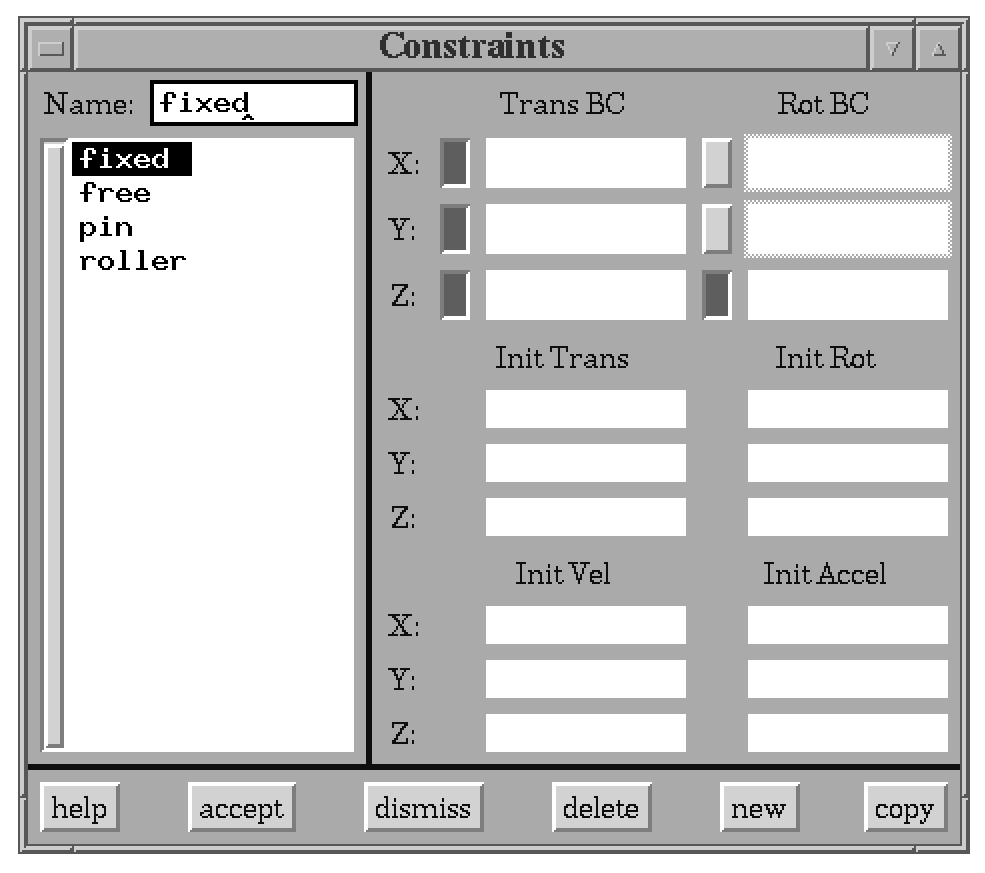
\includegraphics[width=3.45in]{figures/velvet_constraint}
\end{center}
\caption{The constraint dialog box.}
\label{velvet.constraint}
\end{figure}

Selecting an entry in the list will display
the definition for that object and it will instantly make that object the 
active definition for that kind of object.  It would remain active even if 
you were to dismiss the dialog box.  You can use the name field to either set
the name when you are defining a new object or to rename an already defined
object.  For example, if you bring up the material dialog in a
brand new problem, you will be faced with a completely blank slate.  You
can name your first material {\tt aluminum}, 
define some material properties and
click {\bf accept}.  This would register {\tt aluminum}
as an available material and
set it as the currently active material.  Now you want to define another 
material property, say {\tt springy}.  You have two options.  
Clicking {\bf new}
will clear out all of the property fields and the name field and you
can name the new material {\tt springy} and define its properties.  
Alternatively,
you can click {\bf copy} and only the name field will be cleared.  This is 
simply a convenient way to define a new material with properties similar
to the previous material.  All you have to enter are a new name and any
changed or additional material properties.
In either case, you need to click {\bf accept} to register {\tt springy}
as a new material.  If you still want {\tt aluminum} 
as the active material, you simply have to select {\tt aluminum} in the list 
after you have accepted {\tt springy}.  Finally, if you really meant to 
refer to {\tt aluminum} by the name {\tt steel}, you can simply change the name
in the field above the list and click {\bf accept}.  It is important to
note that the basic behavior of these buttons is exactly the
same in all four dialogs.  Only the object specific information
(discussed in more detail below)
in the right side of each behaves differently.

To delete an object you can simply click {\bf delete} in the appropriate
dialog box.  Note that {\em velvet} will not let you delete an object that 
is currently assigned to an element or node.  Clicking and holding the 
{\bf help} button will display a brief help
message for the given dialog box.  

The advantage to this mode of working with objects is that these dialogs
can be left up throughout your work session.  You can have them up and
easily change the active object for a given type.  There is no need
to be constantly popping things up, selecting something or changing
something and then popping it down again only to need it again in 30
seconds.   If you're sure you won't be needing them after some initial
setup, you can safely dismiss them if you don't like too much screen
clutter.  

\subsubsection{The material dialog}

The object specific information for a material property is simply
entered through the labeled text boxes to the right of the material list
(Figure~\ref{velvet.material}).
Additional help regarding each property, including a list of which 
elements require that property to be defined, can be gotten by clicking
on the label for the given property (i.e., click on {\tt E} for
a description of Young's modulus).  If a field is left blank, that
property will be taken as 0.0.

\begin{figure}
\begin{center}
 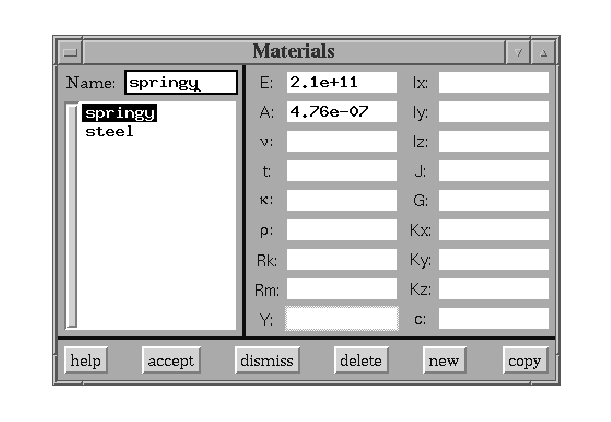
\includegraphics[width=3.38in]{figures/velvet_material}
\end{center}
\caption{The material dialog box.}
\label{velvet.material}
\end{figure}

\subsubsection{The constraint dialog}

The six toggle buttons shown in Figure~\ref{velvet.constraint}
allow you to specify which DOFs are constrained by a boundary condition.  
If a toggle button is engaged, the corresponding text field will also
be used in constructing the boundary condition definition.  If a button is
engaged and the text field is blank, that DOF will be fixed; if a button
is engaged and that field contains the word {\tt hinged} then that
DOF will be treated as a hinge (remember, hinged DOFs only make sense
on certain element types); if a button is engaged and the text field
contains a number, then that DOF will be defined as a displacement boundary
condition; if a button is engaged and the corresponding text field has a
time-dependent expression then that DOF will be treated as time-varying BC.
Finally, if a button is not engaged, then that DOF will remain
completely unconstrained.

Initial conditions for transient analysis problems are defined
with the initial displacement, velocity, and acceleration entries.  For 
initial displacement and velocity conditions
empty entries are taken as 0.0.  For initial acceleration conditions, empty
entries are undefined.  The distinction is that if all of the initial
accelerations are undefined then the mathematical engine will solve for
an initial acceleration vector based on the initial displacement and velocity
vectors.  If any of the initial accelerations are specified in a problem then
any others which were left undefined will be taken as 0.0 and the mathematical
engine will use this vector as the initial acceleration.

\subsubsection{The force dialog}

The two toggle buttons at the top of the dialog toggle the display of force
information between the time domain forces ({\tt Fx \ldots Mz} in a 
\felt{} file) and frequency domain spectral inputs ({\tt Sfx \ldots Smz} in
a \felt{} file).
Forces and moments (or spectra of forces and moments) in each of the three 
directions can be entered in
the appropriate text field.  If an entry is left blank that component
of the force will be taken as 0.0.  The dialog pictured in 
Figure~\ref{velvet.force} is from a model of a bicycle in which there are
two static forces defined.  Just like in a \felt{} file, forces
can be a time- or frequency-dependent function using the independent
variables {\tt t} and {\tt w}.

\begin{figure}
\begin{center}
 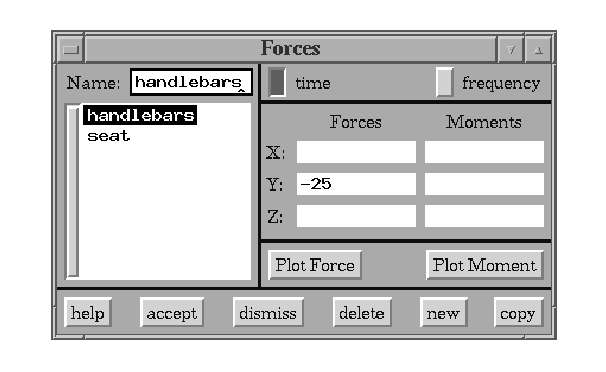
\includegraphics[width=3.16in]{figures/velvet_force}
\end{center}
\caption{The force dialog box.}
\label{velvet.force}
\end{figure}

\subsubsection{The load dialog}

Figure~\ref{velvet.load} shows what the load dialog box looks like after
we have defined both of the distributed loads used in our sample problem.
The eight toggle buttons define the direction of the load.  Note that these
toggles function as a radio group, i.e., only one of them can be
selected at any one time.  The text fields allow you to enter
node, magnitude pairs much the same way that you would define a load in a
standard \felt{} input file. Remember that the node specification refers
to the local element number (i.e., 1 or 2 for a beam, 1, 2 or 3 for a CST, 
etc.)  Also, it is always your responsibility to make sure that 
the loads assigned to an element have a valid direction and node ordering
for that element type.

\begin{figure}
\begin{center}
 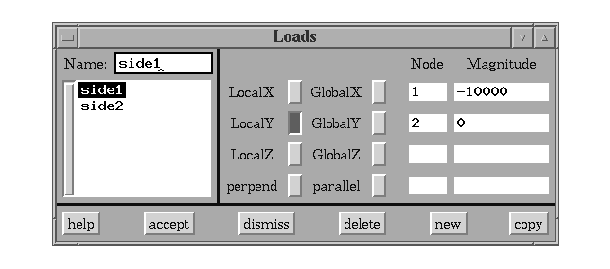
\includegraphics[width=4.06in]{figures/velvet_load}
\end{center}
\caption{The load dialog box.}
\label{velvet.load}
\end{figure}

\subsection{Working with nodes and elements}

The first step in actually laying out the geometry of a problem is usually
to lay the nodes out (elements have to be attached to nodes after all).
Let's assume that we went through everything above and defined 
all the materials, constraints, and loads in our sample problem (there are 
no forces).  We made {\tt steel} the active material and {\tt free} the
active constraint (we'll deal with the loads later).  Now to add a node
all we have to is select {\bf add} from the {\bf node} menu.  
You choose the location of the node simply by clicking in the drawing area.  
A node will be 
created at that location (or the nearest snapped location if snap is on).  
Alternatively, you can specify the exact coordinates within the command 
window.  You do not need to select {\bf add} for each individual node.
Once selected, you are effectively in add node mode and can simply
add additional nodes by repeatedly clicking or typing coordinates.  To stop
adding nodes click on the {\bf quit} or {\bf abort} button in the main
control area.  Most other command functions available from the main
control area will be greyed out while you add nodes.  
In our sample problem all we need to do is click on the
location of our four nodes.  Nodes will be numbered consecutively in 
the order in which they were added.

Once the nodes are down, we need to remember that all four have the
constraint {\tt free} assigned to them (it was active when we added them).  
So now we change the active constraint to {\tt pin} by clicking it in
the constraint list, select {\bf constraint} from the {\bf apply} menu
and click on node 1.  We make node 3 a {\tt roller} by selecting {\tt roller}
on the constraint list and applying it to the node via the apply
mechanism.  Similarly for the fixed condition on node 4.
We could have gotten around this by simply changing the active
constraint before we added each node.  All we would have needed to do was
leave the constraint dialog up and click on the appropriate entry in
the constraint list before we added the node that used that constraint.

Before we can add the elements, we need to know how to set the element
type.  Like an active object, we have to set a current element type before
we can actually add any elements.  There is a distinction, however, as
we cannot go back and apply a different element type to an element.  The
only way to change the type of a given element is to delete it and add
a new element.  We set the current element by choosing {\bf set type}
from the {\bf elements} menu.  This will bring up a dialog similar to
the standard file selection mechanism.  Like the object dialogs, the
element selection dialog can be left up throughout your work session.  
The current element type can be set simply by clicking on the appropriate
name in the list.  The {\bf accept} button is simply there in case you
want to type in the element name.  Typing {\tt beam3d} in the text field
and clicking {\bf accept} is equivalent to simply clicking on the
{\tt beam3d} entry in the list.

Given this mechanism, the logical way to add the elements in our sample 
problem is to set the current element type to {\tt beam} and add elements 1
and 2.  Elements are added by selecting {\bf add} from the {\bf elements}
menu and then clicking on nodes in the appropriate order, or 
entering node numbers in the command window.  {\em velvet} will wait
until you have selected the appropriate number of nodes for the current
type of element before it prompts you to add the next element.
Click {\bf quit} to stop adding elements.  Click {\bf abort} if you
goofed up on an element and just want to start over for that element (e.g.,
if you entered the first two nodes wrong on a CST element).

Once elements 1 and 2 are added we can change the element type to truss
and add element 3 by clicking on nodes 2 and 4.  Before we did this we
would probably also change the active material to {\tt springy} (or we could
just change it with {\bf material} from the {\bf apply} menu later).

We also still need to apply the distributed loads.  All we have to do is
set {\tt side1} active by clicking it in the load dialog and apply it to 
element 1 from the {\bf apply} menu.  Then we do the same thing for
{\tt side2} and element 2.

Deleting nodes and elements (via {\bf delete} under the appropriate menu) must 
proceed in reverse order of adding nodes and elements.  That is, a node can
not be deleted if an element is still attached to it, so the element must be 
deleted first.  Elements can be deleted freely.  Deleting multiple nodes and 
elements is accomplished by clicking on one after the other ({\bf quit}
or {\bf abort}
will finish deleting) or by clicking and holding the middle mouse button and 
dragging out a box containing the nodes or elements to be deleted.  As in 
deleting one at a time, none of the selected nodes which are still attached to 
elements will be deleted.	

\section{More on nodes and elements}
\subsection{Editing nodes}
In addition to simply adding and deleting nodes, {\em velvet} provides
a powerful mechanism for displaying and editing all of the information
about a node.  The node dialog box is shown in Figure~\ref{velvet.node}.  
You can raise this dialog either by selecting {\bf edit} from the 
{\bf node} menu or by clicking directly 
on the node which you want to edit with the left mouse button.  You may want
to use the former option (even though it seems a bit clumsier) in cases
where you can't quite click on the right node.  If you proceed from the
menu option, you will be prompted to either select the node with the mouse
or to type the node number into the command window.  Once the dialog
is up you can change the displayed node either with the arrow keys in the
dialog box, by clicking on a different node in the drawing area or by selecting
a new node through the {\bf edit} option under the {\bf node} menu.
As a third option for editing nodes you can click on a node with the
third mouse button -- this will raise the node editing dialog and the
constraint and force (if appropriate) dialogs with the assigned objects for 
the selected node already highlighted.  This is an easy way to take
a complete look at a given node; remember, however, that any changes you make
to the node's objects will also affect any other nodes that have that
object assigned to them.

\begin{figure}
\begin{center}
 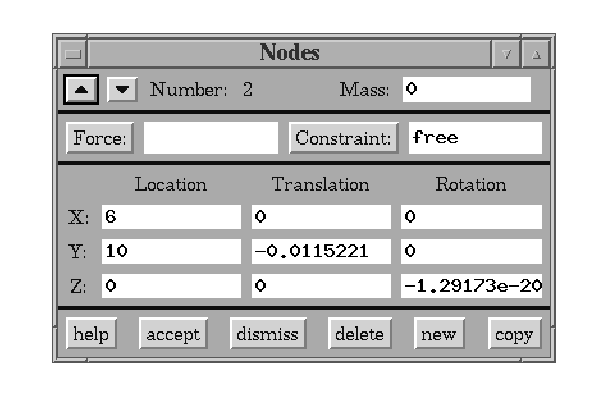
\includegraphics[width=2.91in]{figures/velvet_node}
\end{center}
\caption{The node information and editing dialog.}
\label{velvet.node}
\end{figure}

The information available in the node dialog are the exact nodal
coordinates, all six nodal displacements (valid only after a problem
has been solved), the lumped mass for the node, the name of the 
constraint applied to the node
and the name of the force (if any) applied to the node.  The location,
lumped mass, constraint and force can be modified simply by editing the 
information in this dialog box. To change the applied constraint, you
can enter a new name into the text field or you can click on the 
{\bf constraint} label to pop-up a menu that will
let you choose from a list of the currently defined constraints.  The same
is true for forces by clicking on the {\bf force} label.  Note that while
you can change the applied force on a node via the {\bf force} option under the 
{\bf apply} menu, editing the information in this dialog is the only way to
completely remove the applied force on a node.  Just like the 
object dialogs you need to click {\bf accept} to make your changes
effective.  The rest of the buttons on the bottom of the node dialog also
behave exactly the same as the buttons on the object dialogs.  

{\em velvet} provides two ways for you to change a node's location.  The
first is by changing the location fields in the node dialog.  The second
is by selecting {\bf move} from the {\bf node} menu.  You can then select
the node that you want to move by clicking on it, move to the new location
and click again to put it back down.  Alternatively, just like you can click
the first mouse button on a node to edit, you can click
on a node with the second mouse button to pick it up, move to a new location
and click again with the second mouse button to put it back down. Note that
because {\em velvet} is basically a package for working with two-dimensional
problems, you cannot change the z coordinate of a node in the coordinate
entry fields of the node dialog.

\subsection{Automatic node renumbering}
\label{velvet.renumbering}
{\em velvet} gives you two ways to optimize the node numbering in terms
of reducing the profile of the global stiffness matrix.  The first way
is to select {\bf renumber perm} from the {\bf nodes} menu.  This will actually
rearrange all of the node numbers in the current problem - permanently.
Generally you would choose this option where the node numbering was not
particularly important to your own understanding of the problem.  This might
be the case if the elements had been automatically generated.  If, on the
other hand, you have a paper sketch of the problem which you used to
setup the problem then you may not want to lose that particular node numbering
scheme.

In this latter case what you can do is toggle temporary renumbering by 
selecting {\bf renumber temp} from the {\bf nodes} menu.
This toggle is equivalent to the {\tt -renumber}
command line switch in the command line application {\em felt}.  If this
switch is on, the nodes will be renumbered internally during the computations,
and then restored to their original numbers before you actually see any
output, i.e. the output will reflect the original numbering scheme.  

Both renumbering methods have their advantages.  The permanent scheme reduces
overhead if you will be solving the problem numerous times; do it once
and then why waste the time to figure out that it can't get any better
every time you try to solve it.  The temporary, internal only scheme keeps
the problem and the results referenced the way that you had originally
defined it.  The additional overhead of doing the renumbering each time
can be well worth it for large problems - both in terms of memory
requirements and in solution speed.  For both options, the same caveat applies 
as in the discussion of the command line switch in {\em felt} - 
for small problems, the algorithm probably won't be able to do much
if anything in terms of profile reduction; in these cases it is probably
easiest simply not to worry about either of the renumbering options.

\subsection{Editing elements}

Editing elements is very similar to editing nodes.  You can either select
{\bf edit} from the {\bf elements} menu (particularly in cases where you
will want to choose the element by typing in its number) or click on 
an element (or its number) with the first mouse button to display the element 
dialog (Figure~\ref{velvet.element}).   
Like the node dialog you can change the displayed
elements either with the up and down arrow buttons or by clicking on
a different element with the first mouse button.  Also just like nodes,
you can click on an element with third mouse button to raise the element
dialog and the object dialogs (materials and loads) with the objects assigned
to that element already highlighted.  Again, remember that any changes to
the assigned objects can affect other elements as well as the element
currently displayed in the element dialog.

\begin{figure}
\begin{center}
 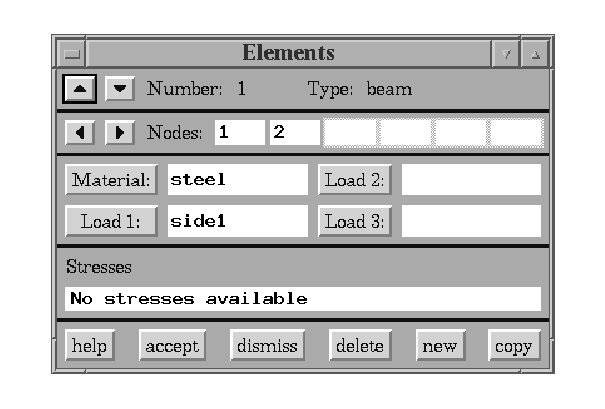
\includegraphics[width=2.95in]{figures/velvet_element}
\end{center}
\caption{The element information and editing dialog.}
\label{velvet.element}
\end{figure}

The information displayed in this dialog includes
the element type, the nodes to which this element is attached, the
material property and distributed loads assigned to this element and,
if the problem has been solved, the stress results for this element.
If an element uses more than
six nodes, you can use the side to side arrow buttons next to the node list
to scroll through them.  
The dialog gives you a simple mechanism for changing the nodes,
material and loads for a given element.  Editing the material and
loads is just like the constraint and force fields in the node dialogs.  You
can either type into the text field or click on the appropriate label
and choose from a menu of currently available objects.  Like forces 
in the node dialog,
changing the information in the element dialog is the only way to 
completely remove all the loads from an element.  Once again of course, you
need to click {\bf accept} to make any changes effective.  The other
buttons across the bottom and their functions 
should be very familiar to you by now.

\section{Using tools}
\label{velvet.tools}

The drawing tools are intended to be aids for meshing up or annotating
a problem.  For instance, you can draw a circle by selecting {\bf circle} from 
the {\bf tools} menu and then place nodes 
along the circle.  The actual figure on the screen does not affect the 
solution of the problem in any way.  {\em velvet} will prompt you in the
command window for the necessary coordinates for each figure type.  As usual,
you can choose coordinates either with the mouse or by typing in the command
window.  In general, however, you must enter all of the coordinate locations
for a given figure with the same input method; what this means is that if
you enter the coordinates of the first point of a line with the keyboard
then you will have to enter the second point with keyboard input as well
or, alternatively, if you select the center of a circle with the mouse then
you will have to select the radius with the mouse as well.

Titles and comments can be entered in the drawing area by selecting
{\bf text} from the {\bf tools} menu
option.  As mentioned earlier, the drawing 
area could then be dumped to an XWD and the result could serve as 
documentation or a figure in a presentation, complete with color annotation.  
Figure~\ref{velvet.tools_pic} shows such a dump with examples of the available
tools.
Tool color and font is controlled from the {\bf configure} option under the 
{\bf canvas} menu.  In addition to text and circles, the {\em velvet} drawing
toolbox currently includes lines, arcs, polylines, and rectangles.

\begin{figure}
\begin{center}
 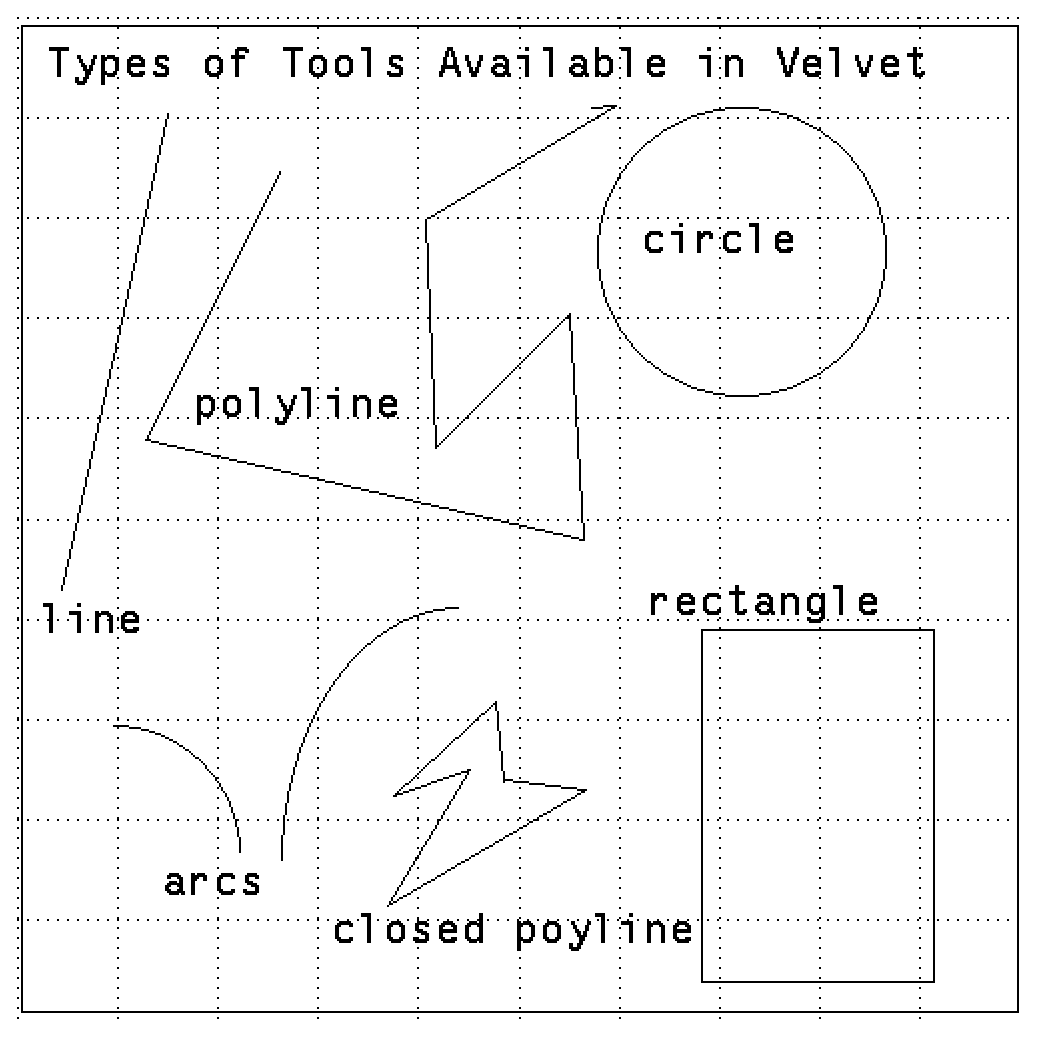
\includegraphics[width=5.5in]{figures/velvet_tools}
\end{center}
\caption{Examples of all the tools available in {\em velvet}.}
\label{velvet.tools_pic}
\end{figure}

To draw a line with the mouse you have to click at the start point and hold
the mouse button while you drag the line to the end point.  Rectangles work
the same way; click and hold while you drag out a box.  For circles your
mouse click will select a center point, and as you move the mouse while
still holding the button, your circle will expand about that center.
When drawing polylines with the mouse, use the first mouse button to
select the starting point by a simple click (not a click and hold).  Additional
end points are defined by additional clicks of the first mouse button.
You can stop adding endpoints by clicking the third mouse button.  If you
want a closed polyline, you can simply click the second mouse button and 
{\em velvet} will draw a line from your current position to the starting
point of the polyline.

Tools can be deleted from the screen just like nodes and elements, either 
one at a time or with a window.  Once in delete mode (select {\bf delete}
from the {\bf tools} menu), individual figures can be selected 
by clicking with the left mouse button or a window can be drawn with the middle 
mouse button.  The delete operation proceeds until {\bf quit} or 
{\bf abort} is clicked.	 Moving a tool figure that already
is drawn on the screen is also straightforward; simply select {\bf move} from 
the {\bf tools} menu, click on the figure that you want to move and then 
click again once you have dragged it to its new location.

The ancillary sections in the \felt{} file that are created when you save a 
problem from {\em velvet}
record all your tool figures.  If these sections are available when you reload
a problem, the tools will automatically be redrawn for you.

\section{Material databases and defaults files}

Often, you will find that certain objects or material properties are being 
used over and over again in different problems.  Dummy \felt{} files can be 
used to make easy use of this repetitive information.  Starting {\em velvet} 
with a \felt{} file that contains a couple of common constraint definitions 
means that those definitions will not need to be specified explicitly within 
{\em velvet} - they will be there for use on start-up.  Similarly for other 
types of objects.  Note that loading a defaults file from within {\em velvet} 
is just like opening a new input file, everything in the current problem will 
be lost.  You can use the {\tt canvas configuration} and {\tt display list}
sections of a \felt{} file to create a custom canvas configuration in a 
defaults file.

Material databases are also special cases of \felt{} input files. They are 
given special treatment within {\em velvet} because they are so convenient.  
Whole classes of material types and shapes (W-shape beams, standard diameter
bars, etc.)  can be stored in a material database and loaded into {\em velvet} 
at any time with the {\bf open database} command under the {\bf file} menu.  
Any changes to material properties or additions of new materials 
can be saved simply by selecting {\bf update database} from the {\bf file} menu.  
The current set of materials is the only thing that is retained when a new 
input file is loaded or a new problem is started within {\em velvet}.	

\section{Automated element generation}

Velvet can generate grids and triangular meshes automatically.  A grid
is defined as an $n \times m$ array of two-dimensional line or quadrilateral
elements.  A
triangular mesh is an arbitrary polygonal shape (possibly with interior
holes) discretized into two-dimensional triangular elements.  When you
select {\bf generate} from the {\bf elements} menu, the type of
generation is automatically determined from the current element type.
Because
both nodes and elements will be generated, both a constraint and a
material property must be active.  You should make sure that the active
object of each type will be appropriate for the majority of nodes and
elements that will be generated.  This will save you from applying a lot of
objects individually once the generation is complete.

\subsection{Generating a grid of line or quadrilateral elements}

Generating a grid requires that you complete the form pictured in
figure~\ref{velvet.grid}.  The entries in the form match parameters
in the {\em corduroy} input syntax (see chapter~\ref{corduroy}).
The x, y, and z start and end locations define the two extreme
corners of the grid.  The number entries set the number of elements
to be generated along each direction and the rule entries set the
spacing rule to be used along each axis.  Rules can either be typed
in or entered by giving the focus to one of the entries and
selecting a rule from the pull-down menu available by clicking on
the {\bf Rule} button.
\begin{figure}
\begin{center}
 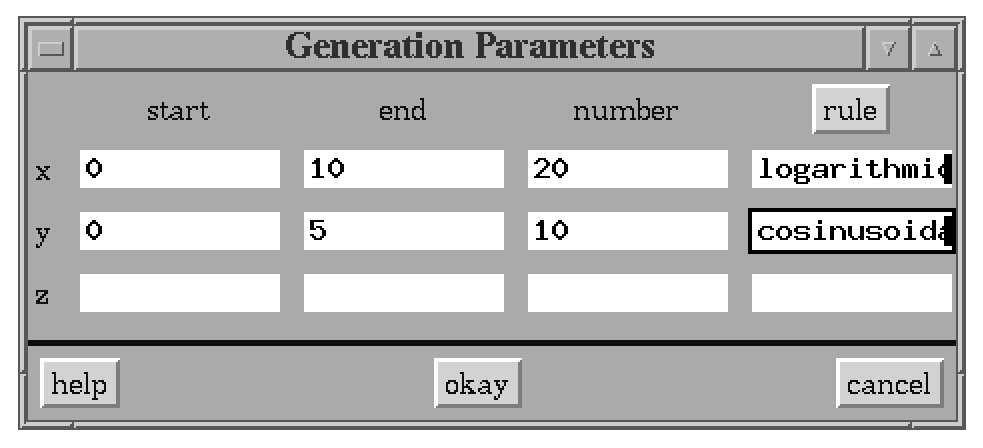
\includegraphics[width=2.9in]{figures/velvet_grid}
\end{center}
\caption{The form for defining line and grid generation parameters.}
\label{velvet.grid}
\end{figure}


\subsection{Generating a mesh of triangular elements}

Generating a mesh of triangles requires a little more work on your part,
but it is still a lot easier than meshing any sort of complicated
geometry (and most simple geometries even) by hand.  When triangles are
being generated a form will pop-up (Figure~\ref{velvet.trimesh}) for you
to define the parameters of the generation.  The parameters are
the target number of elements that you want to generate, the $\alpha$
area constraint factor and the number of holes in your generation region.
The area constraint factor is defined as
\begin{equation}
A_{\rm elt} \leq {\alpha A_{\rm region} \over {\rm target}},
\end{equation}
where $A_{\rm region}$ is the total area of the generation region and
$A_{\rm elt}$ is the maximum area of a generated element.
%
\begin{figure}
\begin{center}
 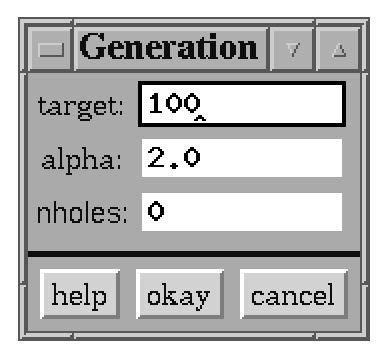
\includegraphics[width=1.07in]{figures/velvet_trimesh}
\end{center}
\caption{The form for defining triangle generation parameters.}
\label{velvet.trimesh}
\end{figure}

Once the parameters are defined, click {\bf okay} to begin defining the 
boundaries of your problem.   Regions are defined by 
putting down marker points in the drawing area (they must be put down in a 
counter-clockwise order).  To finish the boundary, click on the {\bf quit}
button.  If the number of holes was greater than zero then each hole must be 
defined just like the boundary was defined -- by laying down a series of 
marker points -- but in clockwise order.  Each hole is finished by clicking 
the {\bf quit} button. The generation process can be aborted by clicking the 
{\bf abort} button. Typing \key{shift-bkspc} will delete the last marker point 
that was laid down, thus allowing you to correct mistakes without restarting 
the entire sequence.  Once all the regions are defined, {\em velvet} will 
automatically begin generating the mesh.  

\section{Keyboard interface mechanisms}
\label{velvet.keyboard}
\subsection{Keyboard shortcuts}

As in most graphical environments, the pointer can only do so much for you;
often it will be easier for you to use the keyboard.  True, you could get
away with using the mouse for everything, 
but in the long run you will work more efficiently if you learn the 
keyboard interface mechanisms. 

There are two basic ways that you can use key presses in place of mouse
clicks.  The first are commonly called keyboard shortcuts.  This means
that rather than selecting {\bf solve} from the {\bf problem} menu,
you can simply press \key{ctrl-v}.  A complete list of these shortcuts
is given in the quick reference table at the end of this section.

The second common way to use the keyboard is to move through groups of
buttons and text fields with \key{tab} to change the input focus and use
\key{space} to activate the button or change the toggle state.  This is
a very convenient way of working with dialog boxes like the object
dialogs (forces, materials, constraints, loads), the file selection
dialog, the node and element dialogs, the configure dialog, the
triangular mesh parameter dialog and the solution dialog.  When one of
the dialogs has the window manager focus there are a few special keyboard
shortcuts that you can use as well.  \key{ctrl-h} is equivalent to {\bf
help}, \key{return} is {\bf accept} or {\bf okay}, \key{esc} is {\bf
dismiss} or {\bf cancel}, \key{ctrl-d} is {\bf delete}, \key{ctrl-n} is
{\bf new}, and \key{ctrl-c} is {\bf copy}.

\subsection{Command names}

All of the commands that are available through menu options in the main
control area are also available by typing a text command into the command
window at the bottom of the main window.  To use a text command simply
type it into the command window and hit \key{return}.  If you just type
\key{return} with no command entered, {\em velvet} will repeat the 
last command that you entered.  The following table lists
the equivalencies for each command.  The first column lists the name of
the menu button in the control area, the second lists the applicable
entry under that menu, if any, and the third lists the command name(s)
that perform the same action.  The fourth column provides additional
ways that you can perform the same function, either through a keyboard 
shortcut or through mouse interaction with the drawing area.  

{\scriptsize
\begin{center}
 \begin{tabular}{p{1in}p{1.25in}p{1.75in}p{1.5in}} 
\hline
Menu	& Command	& Text command & Other alternatives\\
\hline
File		& New		& \tt new 		& Ctrl-f n \\
		& Open		& \tt open 		& Ctrl-f o \\
		& Save		& \tt save 		& Ctrl-f s \\
		& Save as	& \tt save as 		& Ctrl-f w \\
		& Restore	& \tt restore 		& Ctrl-f r \\
		& Open database & \tt open database 	& \\
		& Update database & \tt update database	& \\
		& Exit		& \tt exit		& Ctrl-f x \\
Solutions	& Solve		& \tt solve 		& Ctrl-v \\
                & Animate       & \tt animate           & \\
		& Results/Output & \tt define output 	& \\
                & Problem/Analysis & \tt define problem & \\ 
Postprocess	& Plot stresses & \tt plot stresses	& \\
		& Plot displacements & \tt plot displacements & \\
		& Plot structure & \tt plot structure 	& \\
		& Contouring 	& \tt contour		& \\
		& Wireframe	& \tt wireframe		& \\
Canvas		& Configure	& \tt configure 	& \\
		& Color control & \tt colors            & \\
		& Zoom to fit   & \tt zoom all 		& Ctrl-Z \\
		& Zoom window	& \tt zoom 		& Ctrl-z \\
		& Save canvas	& \tt dump		& \\
		& Snap		& \tt snap 		& Ctrl-s \\
		& Grid		& \tt grid 		& Ctrl-g \\
		& node numbering & \tt node numbers 	& Ctrl-n \\
		& element numbering & \tt element numbers & Ctrl-e \\
Apply		& Materials	& \tt apply material 	& Ctrl-a m \\
		& Forces	& \tt apply force	& Ctrl-a f \\
		& Constraints	& \tt appply constraint & Ctrl-a c \\
		& Loads		& \tt apply load	& Ctrl-a l \\
Tools		& Circle	& \tt draw circle 	& Ctrl-t c \\
		& Arc		& \tt draw arc 		& Ctrl-t a \\
		& Rectangle	& \tt draw rectangle 	& Ctrl-t r \\
		& Polygon	& \tt draw polygon 	& Ctrl-t p \\
		& Line		& \tt draw line 	& Ctrl-t l \\
		& Text		& \tt draw text 	& Ctrl-t t \\
		& Delete	& \tt delete tool 	& \\
		& Move		& \tt move tool		& \\
Nodes		& Add		& \tt add node 		& \\
		& Edit		& \tt edit node		& button 1 on node \\
		& Delete	& \tt delete node	& \\
		& Move		& \tt move node		& button 2 on node \\
                & Lumped mass   & \tt lumped mass       & \\
                & Renumber perm & \tt renumber nodes    & \\
		& Renumber temp & \tt toggle renumber	& \\
Elements 	& Add		& \tt add element 	& \\
		& Edit		& \tt edit element 	& button 1 on element \\
		& Set type	& \tt set element 	& \\
		& Generate	& \tt generate 		& \\
Materials	&		& \tt edit material 	& Ctrl-d m \\
Constraints	&		& \tt edit constraint 	& Ctrl-d c \\
Forces		&		& \tt edit force 	& Ctrl-d f \\
Loads		&		& \tt edit load 	& Ctrl-d l \\
Quit		&		&			& Esc or button 3 \\
Abort		&		&			& Ctrl-c \\ 
 \end{tabular}
\end{center}}

%%%%%%%%%%%%%%%%%%%%%%%%%%%%%%%%%%%%%%%%%%%%%%%%%%%%%%%%%%%%%%%%%%%%%%%%%
\section{Command line options}
Some of the above functionality can be enabled, disabled or altered via
command line switches when you invoke {\em velvet}.  In addition
to the standard X toolkit options ({\tt -display}, etc.) you can
use any of the following to control the behavior and set the start-up
condition of {\em velvet}.  Each of these options can also be set through
your Xresources using the associated resource name.  

\begin{dispitems}
\item[\tt -sensitive]
Enable sensitive/insensitive menu switching.  {\em velvet} has two major
modes of operation, normal mode and edit mode.  Each mode allows only certain
operations to be performed.  This option allows disabling of the menus
controlling the inactive operations.  This is the default behavior but
may be inappropriate on a slow server.  Associated resource: 
{\tt *sensitiveMenus}.

\item[\tt +sensitive]
Disable sensitive/insensitive menu switching.  Associated resource:
{\tt *sensitiveMenus}.

\item[\tt -numbers]
Enable element and node numbering on start-up.  This is the default
behavior. Associated resource: {\tt *numbers}.

\item[\tt +numbers]
Disable the drawing of element and node numbering on start-up.   On some
servers the node and element numbers may take some extra time to
draw on big problems and since you'll probably turn them off anyways to
reduce clutter, you can use this switch to disable them from the start.
Associate resource: {\tt *numbers}.

\item[\tt -nodeColor color]
Sets the color of nodes and node numbers.  The default color is {\tt blue}.
Associated resource: {\tt *nodeColor}.

\item[\tt -elementColor color]
Sets the color of elements and element numbers.  The default color is 
{\tt black}.  Associated resource: {\tt *elementColor}.  

\item[\tt -toolColor color]
Sets the color of tools (rectangles, lines, circles) and interactive windows.
The default color is {\tt red}.  Associated resource: {\tt *toolColor}.

\item[\tt -labelFont font]
Sets the font used for node and element numbers.  The default font is 
{\tt 5x8}.  Associated resource: {\tt *labelFont}.

\item[\tt -toolFont font]
Sets the font used for text drawn using the tools.  The default font is
{\tt fg-22}.  Associated resource: {\tt *toolFont}.

\item [\tt -cpp filename]
	substitute {\tt filename} for the pre-processor to run on the 
	input file.

\item [\tt -nocpp]
   	do not run the input file through the pre-processor.

\item [\tt -Idirectory]
	add {\tt directory} to the standard search path for include files in
	the pre-processor.

\item [\tt -Uname]
   	undefine the macro {\tt name} in the pre-processor.

\item [\tt -Dname=value]
	define {\tt name} to be the macro {\tt value} in the pre-processor.
\end{dispitems}
